\documentclass[10pt, a4paper,spanish]{article}

\usepackage{./mystyle}
\usepackage{./myvars}



%-----------------------------

\begin{document}

	\maketitle % Insert title

	\thispagestyle{fancy} % All pages have headers and footers


%-----------------------------
%	ABSTRACT
%-----------------------------

	\begin{abstract}
		\noindent En este documento se ha analizado el comportamiento de los algoritmos \emph{ID3} y \emph{J48} a través de su implementación en la herramienta de minería de datos \emph{Weka}\cite{tool:weka}. Como caso de prueba se ha entrenado a partir de la tabla de verdad de una función lógica a los distintos algoritmos. Como resultados de dicho análisis se ha comprobado el sobreajuste producido por \emph{ID3}, que en este caso proporciona mejores resultados que \emph{J48} debido al carácter finito de la función así como la estrategia de entrenamiento y test seguida para la realización de la comparativa.
	\end{abstract}

%-----------------------------
%	TEXT
%-----------------------------


  \section{Tómese la siguiente función lógica y obténgase el árbol de decisión correspondiente usando WEKA\cite{tool:weka}}

		\begin{equation}
			\label{eq:logic_equation}
			\neg(A \land B) \lor \neg(C \land D) \oplus E
		\end{equation}

		\paragraph{}
		En esta práctica se ha generado la tabla de verdad de la función descrita en la ecuación \eqref{eq:logic_equation}. Por lo tanto, el conjunto de datos que se ha utilizado en este caso sigue la siguiente estructura:
		\begin{enumerate*} [label=\itshape\alph*\upshape)]
			\item los atributos de cada dato se corresponden con una determinada combinación de las variables de entrada de \eqref{eq:logic_equation},
			\item mientras que el valor de la clase será el valor de verdad de dicha combinación.
		\end{enumerate*}

		\paragraph{}
		El conjunto de datos está compuesto por tanto, por 5 atributos de tipo booleano (discretos) al igual que la clase, que también es de tipo booleano. Puesto que la función está formada por 5 argumentos y cada uno de ellos puede tomar 2 valores, nuestro conjunto de datos está formado por $2 ^ 5 = 32$ datos. Todos ellos han sido recogidos en la tabla \ref{eq:truth_table}. Dicha tabla de verdad ha sido generada a partir de la clase \emph{LogicDataSet} codificada en el lenguaje \emph{Python}, a la cual se puede acceder a partir de \url{https://github.com/garciparedes/python-examples/blob/master/data_sets/logic_data_set.py}\cite{github:garciparedes-python-examples}.


		\paragraph{}
		El propósito de esta práctica es analizar el comportamiento de las estrategias de aprendizaje automático básadas en estructuras jerárquicas (árboles). Para ello se ha utilizado la herramienta \emph{Weka}\cite{tool:weka}, que permite la realización de diversas tareas relacionadas con el aprendizaje automático de manera simple y de manera gráfica sobre conjuntos de datos. En este caso se ha realizado una comparativa entre los algoritmos de clasificación basada en árboles mediante aprendizaje supervisado.

		\paragraph{}
		Debido a la naturaleza intrínseca de un estructura en forma de árbol, esto permiten la representación de funciones lógicas con un alto grado de acierto. Para comprobar dicha cualidad, se ha realizado un ánalisis de resultados de los algoritmos \emph{ID3} y \emph{J48}, cuyas diferencias son las siguientes:

		\begin{itemize}

			\item \textbf{ID3}: Es el algoritmo básico de generación de árboles de decisión a partir de un conjunto de datos formado tanto por atributos como valores de clase de carácter discreto. Utiliza heurísticas basadas en la Teoría de Información. Debido a sus simplicidad, está muy condicionado al conjunto de datos de entrenamiento.

			\item \textbf{J48}: Es la versión implementada en el lenguaje \emph{Java} del algoritmo \textbf{C4.5}, una versión con numerosas mejoras respecto de \emph{ID3}, tales como:
				\begin{enumerate*}[label=\itshape\alph*\upshape)]
					\item la capacidad de procesar atributos continuos mediante la generación,
					\item manejo de valores desconocidos,
					\item tratamiento de mismos atributos de entrada para distintos valores para la clase de destino y
					\item poda para tratar de evitar el sobreajuste.
				\end{enumerate*}
		\end{itemize}

		\paragraph{}
		Para los casos de prueba, con los dos algoritmos se han utilizado los parámetros por defecto de la herramienta \emph{Weka}\cite{tool:weka}. Tras utilizar todo el conjunto de datos tanto para entrenamiento como para test, los árboles generados por el algoritmo \textbf{ID3} y \textbf{J48} se muestran en las figuras \ref{fig:id3-tree} y \ref{fig:j48-tree}. Dichas figuras han sido generadas a partir de la herramienta \emph{treetograph}\cite{github:ismtabo-treetograph}.


		\subsection{Resultados obtenidos a partir de \emph{ID3}}

			\paragraph{}
			El algoritmo \emph{ID3}, tal y como se ha dicho en el párrafo anterior, ha generado el árbol de la figura \ref{fig:id3-tree}. Tal y como se puede apreciar, este ha tenido en cuenta todos los datos para generar el árbol, por lo cuál tiene la misma profundidad que el número de atributos del conjunto de datos. Esto es equivalente al número de variables que tiene la función lógica \eqref{eq:logic_equation} que se ha querido representar.

			\begin{figure}[h]
				\begin{center}
					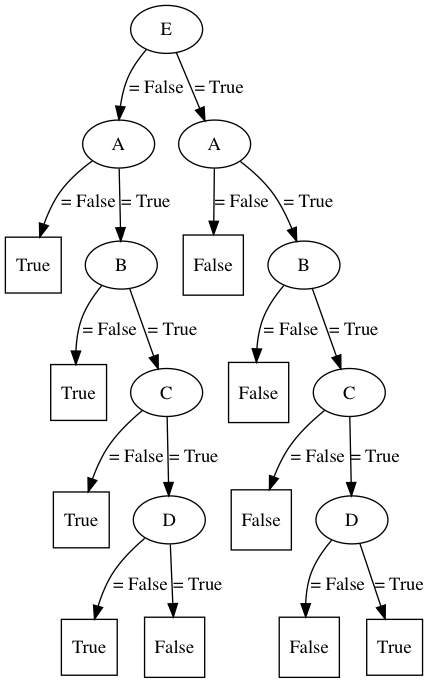
\includegraphics[width=0.5\textwidth]{id3-tree}
				\end{center}
				\caption{Árbol de decisión generado a partir del algoritmo \emph{ID3}}
				\label{fig:id3-tree}
			\end{figure}

			\paragraph{}
			Como consecuencia de dicho tamaño, con esta alternativa se consigue la matriz de confusión de la tabla \ref{table:confusion-matrix-id3}. Como vemos, esta muestra que la tasa de acierto del árbol es del $100\%$, ya que este captura todas las posibles combinaciónes de la función lógica \eqref{eq:logic_equation}. Los valores $p_i$ y $\pi_j$ representan la proporción de aciertos de cada clase y la proporción de muestras de cada clase del conjunto de test respectivamente.

			\begin{table}[h]
				\begin{center}
					\begin{tabular}{r c c|c|l}
						& & \multicolumn{2}{ c }{Valor Real} \\ \cline{3-4}
						& & \multicolumn{1}{ |c| }{Positivo} & \multicolumn{1}{ |c| }{Negativo} & \multicolumn{1}{ c }{$p_j$}\\ \cline{2-4}
						\multicolumn{1}{  c  }{\multirow{2}{*}{Valor Predicho} } 	& \multicolumn{1}{ |c| }{Positivo} & $16$ & $0$ &  $1$   \\ \cline{2-4}
						\multicolumn{1}{  c  }{}                        					& \multicolumn{1}{ |c| }{Negativo} & $0$  & $16$ & $1$ \\ \cline{2-4}
						& \multicolumn{1}{ c }{$\pi_j$} & \multicolumn{1}{ c }{$0.5$} & \multicolumn{1}{ c }{$0.5$} & \multicolumn{1}{ c }{$N = 32$}
					\end{tabular}
				\end{center}
				\caption{Matriz de confusión resultante de del conjunto de datos generado a partir de la ecuación \eqref{eq:logic_equation} por el algortimo \emph{ID3}}
				\label{table:confusion-matrix-id3}
			\end{table}

			\paragraph{}
			Los resultados obtenidos han sido tan satisfactorios debido a los siguientes factores:
			\begin{enumerate*}[label=\itshape\alph*\upshape)]
				\item la naturaleza lógica de la función utilizada para generar el conjunto de datos,
				\item la utilización de todo el conjunto de datos tanto para entrenamiento como para test y
				\item la estrategia utilizada por el algoritmo \emph{ID3}, que no restringe el tamaño del árbol generado y captura todas las alternativas que obtiene a partir del conjunto de entrenamiento.
			\end{enumerate*}

		\subsection{Resultados obtenidos a partir de \emph{J48}}

			\paragraph{}
			El algortimo \emph{J48} se diferencia de su versión anterior en que proporciona un mayor número de características, que le hacen más versátil y eficiente a la hora de clasificar conjuntos de datos (a pesar de que en este ejemplo se haya producido el fenómeno contrario). En este caso, el algoritmo ha generado un árbol de decisión de altura 1, es decir, tan solo basará la clasificación en el valor de 1 único atributo del conjunto de datos, o lo que es lo mismo, 1 de las variables de la función lógica \eqref{eq:logic_equation}. Esto se ilustra gráficamente en la figura \ref{fig:j48-tree}

			\begin{figure}[h]
				\begin{center}
					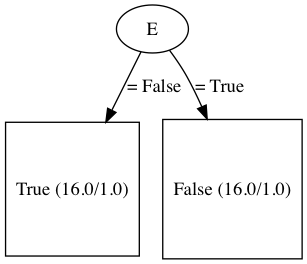
\includegraphics[width=0.5\textwidth]{j48-tree}
				\end{center}
				\caption{Árbol de decisión generado a partir del algoritmo \emph{J48}}
				\label{fig:j48-tree}
			\end{figure}

			\paragraph{}
			La razón por la cual se ha dado este suceso es debido a que el algoritmo \emph{J48} realiza una poda al árbol que previamente genera siguiendo la misma estrategia que \emph{ID3}. Esta poda consiste en eliminar nodos o reducir la altura del árbol basandose en un umbral admisible de pérdida de precisión a la hora de clasificar los datos. La razón por la cual utiliza dicha técnica es para tratar de evitar el sobre-ajuste.

			\paragraph{}
			El sobre-ajuste consiste en un fenómeno que consiste en la sobre adaptación del algoritmo de aprendizaje a los valores de entrenamiento. Lo que conlleva un peor comportamiento cuando se le presentan valores desconocidos (con los cuales no ha sido entrenado). El uso de esta técnica conlleva situaciones como lo ocurrido en este caso, es decir, una mayor tasa de fallo. Esto se puede comprobar a partir de la matriz de confusión de la tabla \ref{table:confusion-matrix-j48}, obtenida tras volver a clasificar los mismos datos con los que previamente ha sido entrenado el algoritmo.

			\begin{table}[h]
				\begin{center}
					\begin{tabular}{r c c|c|l}
						& & \multicolumn{2}{ c }{Valor Real} \\ \cline{3-4}
						& & \multicolumn{1}{ |c| }{Positivo} & \multicolumn{1}{ |c| }{Negativo} & \multicolumn{1}{ l }{$p_j$}\\ \cline{2-4}
						\multicolumn{1}{  c  }{\multirow{2}{*}{Valor Predicho} } 	& \multicolumn{1}{ |c| }{Positivo} & $15$ & 1 &  $0.9375$   \\ \cline{2-4}
						\multicolumn{1}{  c  }{}                        					& \multicolumn{1}{ |c| }{Negativo} & $1$  & 15 & $0.9375$ \\ \cline{2-4}
						& \multicolumn{1}{ c }{$\pi_j$} & \multicolumn{1}{ c }{$0.5$} & \multicolumn{1}{ c }{$0.5$} & \multicolumn{1}{ l }{$N = 32$}
					\end{tabular}
				\end{center}
				\caption{Matriz de confusión resultante de del conjunto de datos generado a partir de la ecuación \eqref{eq:logic_equation} por el algortimo \emph{J48}}
				\label{table:confusion-matrix-j48}
			\end{table}

			\paragraph{}
			En la matriz de confusión de la tabla \ref{table:confusion-matrix-j48} se aprecia que el árbol generado no tiene un comportamiento tan "bueno" como el anterior, produciendo una tasa de acierto de $p = 0.9375$ en ambos casos. Lo cual es debido a la poda del árbol de decisión.


		\subsection{Conclusiones}

			\paragraph{}
			Mediante el ánalisis de resultados de los distintos algoritmos sobre el conjunto de datos generado por una función lógica se ha comprobado que la selección del mejor algoritmo para clasificarlo depende de muchos factores.

			\paragraph{}
			Por tanto, la selección de uno sobre otro muchas veces dependerá del problema que se pretenda resolver, así como el tamaño del conjunto de datos disponible para entrenamiento y la naturaleza del mismo. Además pueden intervenir otros factores como la tasa de acierto que se espera conseguir o las restricciones de carácter computacional que se pretendan imponer (lo cual requiere árboles de decisión de menor tamaño).



			\begin{table}[p]
				\begin{center}
					\csvautotabular{data.csv}
				\end{center}
				\caption{Tabla de verdad de la ecuación \ref{eq:logic_equation}}
				\label{eq:truth_table}
			\end{table}


%-----------------------------
%	Bibliographic references
%-----------------------------
	\nocite{subject:taa}
  \bibliographystyle{acm}
  \bibliography{bib/misc}

\end{document}
